\documentclass[conference]{IEEEtran}
\IEEEoverridecommandlockouts
\usepackage{cite}
\usepackage{amsmath,amssymb}
\usepackage{newtxtext,newtxmath}
\usepackage{graphicx}
\usepackage{textcomp}
\usepackage{xcolor}
\usepackage{booktabs}
\usepackage{url}
\usepackage[hidelinks]{hyperref}
\setlength{\textfloatsep}{6pt}
\setlength{\abovecaptionskip}{2pt}

\begin{document}

\title{From Words to Worlds: Text-to-Image Generation with CLIP-Conditioned Stable Diffusion}

\author{
\IEEEauthorblockN{Sankalp Hegde}
\IEEEauthorblockA{\textit{Northeastern University}\\Boston, MA, USA}
\and
\IEEEauthorblockN{Reshma Jose}
\IEEEauthorblockA{\textit{Northeastern University}\\Boston, MA, USA}
\and
\IEEEauthorblockN{Jairaghavendra Sridhar}
\IEEEauthorblockA{\textit{Northeastern University}\\Boston, MA, USA}
}

\maketitle

\begin{abstract}
This proposal describes our IE 7615 generative project, a text-to-image pipeline that conditions a pretrained latent
diffusion model on Transformer text embeddings. We prepared 4,958 cleaned image-caption pairs from COCO 2017, built a
CLIP embedding baseline, and ran five prompt-to-image tests with Stable Diffusion v1.5.
\end{abstract}

\begin{IEEEkeywords}
text-to-image generation, diffusion models, CLIP, classifier-free guidance
\end{IEEEkeywords}

\section{Dataset}
We use the COCO 2017 validation split (5,000 images, 25,014 human captions). Captions were normalised (whitespace,
punctuation), exact duplicates per image removed, and captions outside 5 to 40 words dropped; every kept caption fits
in CLIP's 77-token context (mean 12.8 tokens). Images were verified, converted to RGB (10 greyscale), filtered for a
short side of at least 256 px (42 removed), then centre-cropped and resized to $512\times512$, the native resolution of
our generator. The result is \textbf{4,958 images with 24,788 captions}; the median-length caption of each image is
its primary prompt, and the real images form the reference set for FID.

\section{Model and Planned Experiments}
\textbf{Generator.} Stable Diffusion v1.5, a latent diffusion model: a VAE maps images to $64\times64\times4$
latents, and a U-Net denoises them while attending, through cross-attention, to the prompt embedding from a frozen
CLIP ViT-L/14 text encoder ($77\times768$, one vector per token). \textbf{Classifier-free guidance} combines the
conditional and empty-prompt predictions,
$\hat\epsilon=\epsilon_\emptyset+w\,(\epsilon_c-\epsilon_\emptyset)$, with guidance scale $w$.
\textbf{Experiments.} We will vary the sampler and noise schedule (DDIM, DPM-Solver, Euler), the number of sampling
steps (10 to 50), and $w$ (1 to 15), and compare conditioning strengths and text encoders (CLIP vs.\ BERT-style
embeddings). \textbf{Evaluation.} FID and Inception Score against our COCO reference images, and CLIP score for
prompt-image alignment. \textbf{Baseline.} CLIP ViT-B/32 embeddings of our pairs are well aligned: matched pairs
reach a cosine similarity of 0.305 vs.\ 0.154 for random pairs, and caption-to-image retrieval gives R@1 of 51.5\% on
1,000 pairs (29.5\% on all 4,958).

\section{Sample Test Runs}
Five prompts (three COCO captions, two new) were generated at $512\times512$ with DPM-Solver, 25 steps, $w=7.5$ and
seed 42, taking about 29~s per image on an Apple M4 GPU (Table~\ref{tab:runs}, Fig.~\ref{fig:samples}). All five are
recognisable, but two show typical conditioning failures: the bananas in prompt 2 are missing, and the frisbee in
prompt 3 is held in front of the dog rather than in its mouth. Generated images even score higher in CLIP score than
the real COCO photos of the same captions, a reminder that CLIP score alone over-rewards text alignment.

\begin{table}[t]
\caption{Five test runs (CLIP score $=100\times$ cosine, ViT-B/32)}
\label{tab:runs}
\centering\footnotesize
\begin{tabular}{@{}c p{0.68\columnwidth} c c@{}}
\toprule
\# & Prompt & Gen. & Real \\
\midrule
1 & A man carrying a bag walking down the train tracks & 28.3 & 27.9 \\
2 & A row of beer bottles and bananas on a wooden counter & 30.2 & 29.1 \\
3 & A large brown dog holding a neon frisbee in his mouth & 36.9 & 31.1 \\
4 & A red vintage bicycle leaning against a brick wall in the rain & 34.5 & -- \\
5 & A watercolor painting of a lighthouse at sunset & 36.3 & -- \\
\bottomrule
\end{tabular}
\end{table}

\begin{figure}[t]
\centering
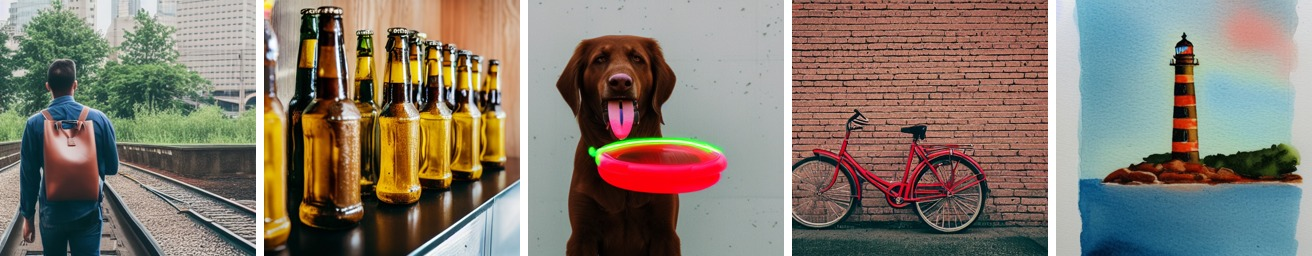
\includegraphics[width=\columnwidth]{../outputs/m1_samples/strip.jpg}
\caption{Generated images for prompts 1 to 5 (left to right).}
\label{fig:samples}
\end{figure}

\section{Team Roles}
\textbf{Sankalp Hegde}: diffusion pipeline and text-encoder integration, sampler and guidance experiments.
\textbf{Reshma Jose}: dataset curation, cleaning and preprocessing, prompt sets.
\textbf{Jairaghavendra Sridhar}: evaluation (FID, Inception Score, CLIP score), results gallery.
All members contribute to the analysis, ethics discussion, report and presentation.

\section{Code Repository}
\url{https://github.com/sankalphegde/ie7615-generative-project}

\end{document}
